% TODO: vllt dieses kapitel auf dateien teilen, is ziemlich lang
In diesem Kapitel werden die zum Verständnis der Implementierung benötigten theoretischen, sowie technischen Grundlagen beschrieben. Dabei werden primär die Funktionalität von \acs{WebRTC} an sich, als auch die damit verbundenen Signal-Mechanismen und Infrastrukturen behandelt.

\section{Echtzeitanwendungen}
Unter den Begriff Echtzeitanwendung fällt prinzipiell jede Anwendung, deren von Nutzern ausgelöste Ereignisse nur gewisse, in der Regel für den Nutzer nicht wahrnehmbare Verzögerungen aufweisen dürfen \cite{realtimeapp}. Ein Beispiel für Echtzeitanwendungen sind Audio- und Videokommunikationsprogramme. Die Audio- und Videodaten müssen schnellstmöglich zwischen den Teilnehmern eines Anrufs ausgetauscht werden, um den Eindruck zu vermitteln, dass die Gesprächsteilnehmer direkt miteinander sprechen. Spricht zum Beispiel eine Person, so muss der Ton zur nahezu gleichen Zeit bei allen anderen Personen, welche dem Anruf teilhaben, ankommen.

\section{Netzwerkarchitekturen}
In dieser Arbeit werden zwei Netzwerkarchitekturen behandelt: Client-Server und Peer-To-Peer Netzwerkarchitekturen.

\subsection{Client-Server-Modelle}
Eine Client-Server Netzwerktopographie setzt sich aus primär zwei Arten an Knoten zusammen: Clients und Servern. Ein Server hat die Aufgabe, den Clients Daten und Services zur Verfügung zu stellen \cite{silveira2015}. In Browsern kann die Websocket-API zur Erstellung von bidirektionalen Client-Server-Verbindungen verwendet werden.\par

%\subsubsection{Web-Architektur}
%Die Architektur von Webanwendungen basiert in der Regel auf auf einem Client-Server-Modell, wobei der Browser des Clients \acf{HTTP}-Anfragen an den Server sendet, um Inhalte vom Server abzurufen. Diese Inhalte lassen sich anhand eines \acf{URI}, beziehungsweise einer \acf{URL} abrufen. Die Webanwendung kann zudem durch JavaScipt-Code mit eingebetteten \acf{API}s der Browser interagieren \cite{loreto2014}.\par

\subsubsection{Authoritative-Server}
Bei der Entwicklung von Mehrspieler-Spielen wird oftmals das sogenannte \glqq{}Authoritative-Server\grqq{}-Modell verwendet. Dabei ist ein Zentraler Server für die gesamte Verwaltung des Spielstandes zuständig. Die Spieler -- die Clients -- halten lediglich den minimal benötigten Status, um das Spiel darzustellen. Jede Aktion des Spielers, welche den Spielstand beeinflusst -- zum Beispiel das Bewegen einer Spielfigur oder das Ziehen einer Karte -- muss über den Server geregelt und autorisiert werden \cite{authservermodel} (vgl. Abbildung~\ref{figure:authserver}).\par

\begin{figure}[h]
\centering
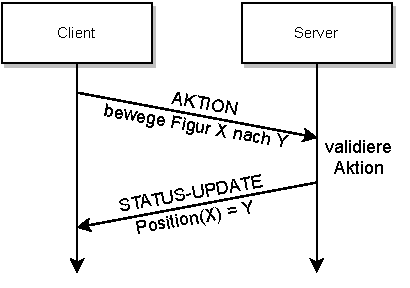
\includegraphics[width=0.65\textwidth]{bilder/PDF_SVG/AUTH_SERVER.pdf}
\caption{Beispielhafte Interaktion in einem Authoritative-Server-Modell.}
\label{figure:authserver}
\end{figure}

Dieser Ansatz eignet sich besonders für Spiele, in welchen Spieler nicht durch unerlaubte Modifikation der Spieldateien Vorteile verschaffen dürfen. Da alle Aktionen über den Server geregelt werden, ist es einfach unerlaubte Änderungen am Spielstand zu verbieten \cite{authservermodel}.\par

\subsection{Peer-To-Peer Netzwerke}
Ein weiterer, gut definierter aber für Browserbasierte Spiele selten verwendeter Ansatz für die Vernetzung von Spielern ist die \acf{P2P}-Architektur. \acs{P2P}-Netzwerke sind dezentralisiert, es existiert kein zentraler Server, die Nutzer (Peers) sind gleichberechtigt und tauschen Daten direkt untereinander aus. Somit ist kein zentraler Server von Nöten, um Daten zwischen Clients weiterzuleiten. Dies führt zu Kostenersparnissen auf Seiten des Anbieters, in Form von weniger Bedarf an Hardware.\par

\section{Network Address Translation}
Aufgrund der Form von \acs{IP}v4-Adressen ist deren Anzahl limitiert. Daher befinden sich viele Geräte in der Regel in einem Subnetz -- einem lokalen \acs{IP}v4-Adressraum -- und nutzen zusammen eine öffentliche \acs{IP}v4-Adresse. \acf{NAT} ermöglicht es den Geräten im Subnetz, Geräte außerhalb des Subnetzes zu erreichen. Router verwalten dazu eine \acs{NAT}-Übersetzungstabelle, mit welcher Nachrichten zwischen externen und internen Geräten weitergeleitet werden \cite{baun}. \acs{NAT}s sind insbesondere bei der Erstellung von \acs{P2P}-Verbindungen problematisch, da ein Gerät von außerhalb sich nicht direkt mit einem Gerät in einem Subnetz verbinden kann \cite{natproblemsRFC}.

\section{Web Real-Time-Communication}
Bei \ac{WebRTC} handelt es sich um einen Quelloffenen Standard zur Echtzeitkommunikation zwischen Browsern. Der Standard ermöglicht es Browsern, welche den \acs{WebRTC} Standard unterstützen, sich ohne zusätzliche Software oder Plugins direkt miteinander zu verbinden. Dies führt in der Regel zu -- im Verlgeich zu Datenaustausch über einen Zentralen Server -- geringeren Latenzen, sowie Kostenersparnissen durch weniger Serverlast. WebRTC ist primär auf Audio- und Videokommunikation ausgelegt, ermöglicht aber auch das Senden von arbitraren Daten.\par

Der Standard wurde zuerst von Global IP Solutions (GIPS) entwickelt. In 2011 erwarb Google GIPS, machte die \acs{WebRTC}-Komponenten Open-Source, und ermöglichte die Integration der Technologie in Web-Browsern durch die Entwicklung einer JavaScript-\acs{API}. Seitdem arbeiten das \acs{W3C} und die \acf{IETF} an der Standardisierung der Java-Script-\acs{API}s \cite{loreto2014}.

Am 26. Januar 2021 veröffentlichte das \acs{W3C} die \acs{WebRTC}-Recommendation -- \acs{WebRTC} ist damit ein offizieller, vom \acs{W3C} und der \acs{IETF} befürworteter Web-Standard, welcher für eine weitverbreitete Verwendung bereit ist. 

\subsection{Aufbau von WebRTC}
WebRTC ist kein proprietärer, einzelner und zusammenhängender Standard, sondern eine Ansammlung bereits existierender Protokolle, Technologien und Standards, welche unter anderem den Aufbau von Verbindungen, Audio- und Videoübertragung, sowie Datenübertragung regeln.\par

\begin{figure}[h]
\centering
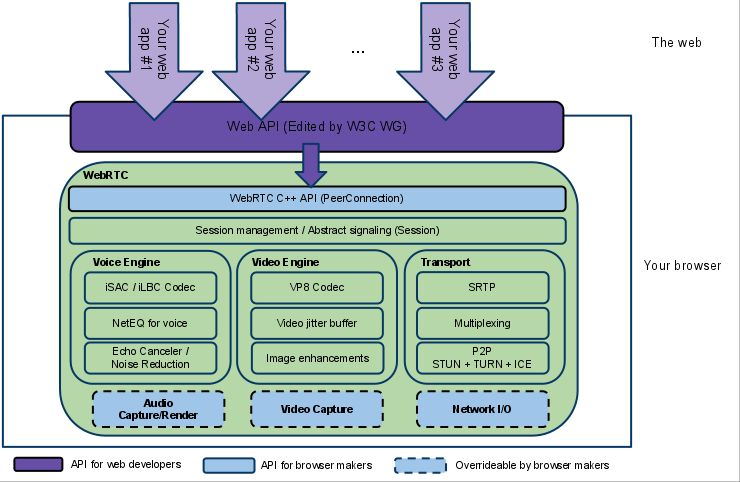
\includegraphics[width=0.95\textwidth]{bilder/webrtc-diagram.png}
\caption{Diagramm der WebRTC-Architektur.}
\source{\url{https://webrtc.github.io/webrtc-org/architecture/}}
\label{fig:webrtcArchitecture}
\end{figure}

Wie dem Architekturdiagramm in Abbildung ~\ref{fig:webrtcArchitecture} zu entnehmen, gliedert sich WebRTC primär in eine Web-\acs{API} und das \acs{WebRTC}-Framework. Hinzu kommen Signalisierungsmechanismen, welche zum Aufbau einer Verbindung benötigt werden. Diese sind nicht durch den WebRTC-Standard vorgeschrieben. Es ist dem Entwickler überlassen, wie die Signalisierung letztendlich implementiert wird -- es muss lediglich möglich sein, Daten zur Sitzunsinitialisierung zwischen jeweils zwei Peers auszutauschen.\par

\subsubsection*{Web-API}
Die Web-\acs{API} setzt sich aus einer Reihe an JavaScript Schnittstellen zusammen. Diese Schnittstellen können auf das unterliegende Framework zugreifen. Primär werden dabei die folgenden Schnittstellen verwendet:

\begin{itemize}
  \item Die \textbf{RTCPeerConnection}-Schnittstelle repräsentiert eine WebRTC-Verbindung zwischen dem lokalen Browser (Local-Peer), und einem externen Browser (Remote-Peer) \cite{rtcpeerconnection}. Die Signalisierungsmechanismen folgen dabei dem \ac{JSEP}, die Verbindung selbst wird via dem \ac{ICE} Framework hergestellt \cite{loreto2014}.
  
  \item Ein \textbf{RTCDataChannel} ist ein, von der RTCPeerConnection erstellter, bidirektionaler Datenkanal, welcher den Austausch von arbitraren Nachrichten zwischen Browsern ermöglicht. Eine RTCPeerConnection kann mehrere Datenkanäle besitzen. Zum Datenaustausch wird das \ac{SCTP} verwendet \cite{loreto2014, rtcpeerconnection}.
  
  \item Die \textbf{MediaStream}-\acs{API} dient dazu, Audio- und Videosignale eines Gerätes abzurufen. Zur Übertragung dieser wird das \ac{RTP}, beziehungsweise das \ac{SRTP} verwendet \cite{loreto2014}.
\end{itemize}

\subsubsection*{WebRTC Framework}
Das \acs{WebRTC}-Framework gliedert sich in Audio- Video- und Übertragungssysteme. Die Audio- und Videosysteme befassen sich dabei unter anderem mit der Abfrage von Audiodaten des Gerätemikrofons oder Videodaten über eine Kamera. Zudem sind diese Systeme für die en- und decodierung von Audio- und Videodaten auf Basis verschiedener Audio- und Videocodecs zuständig. Die Transportsysteme umfassen Protokolle und Systeme, um Sitzungen zwischen Peers aufzubauen, und Daten zwischen den Peers zu auszutauschen.

\subsection{Protokolle}
WebRTC nutzt eine Reihe an Protokollen und Frameworks, um den Sitzungsaufbau, die Verbindung, sowie den Datenaustausch zwischen Peers zu ermöglichen. Der WebRTC Protokollstack ist in Abbildung~\ref{fig:protocols} abgebildet.

\begin{figure}[h]
\centering
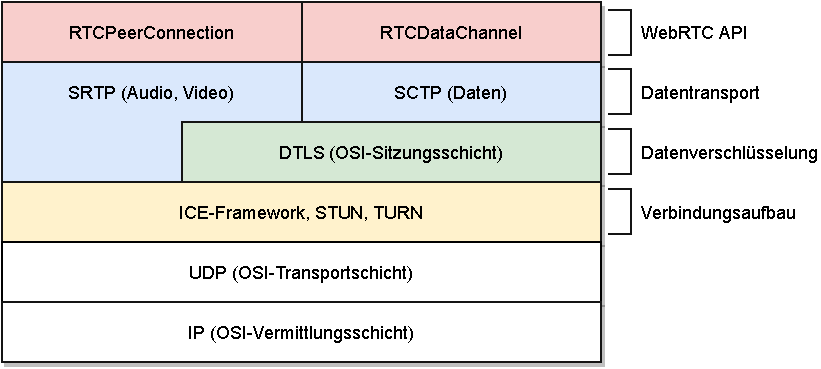
\includegraphics[width=0.78\textwidth]{bilder/PDF_SVG/PROTOCOL_STACK.pdf}
\caption{\acs{WebRTC}-Protokollstack.}
\source{Nach \url{https://webrtc-security.github.io/} (Stand 07.05.2021), Abb. 2}
\label{fig:protocols}
\end{figure}

\subsubsection{JavaScript Session Establishment Protocol}
Die Signalisierungsebene einer \acs{WebRTC}-Anwendung ist nicht vom \acs{WebRTC}-Standard definiert, damit verschiedene Applikationen mitunter verschiedene Signalisierungsprotkolle, wie zu Beispiel das \acf{SIP}, oder ein proprietäres Protokoll nutzen können \cite{loreto2014}.\par

Das \acf{JSEP} erlaubt es einem Entwickler, die volle Kontrolle über die unterliegende Zustandsmaschine des Signalisierungsprozesses zu haben, welche die Initialisierung einer Sitzung kontrolliert \cite{loreto2014}. Eine Sitzung wird immer zwischen zwei Endpunkten etabliert, einem initiierendem Endpunkt, und einem empfangenden Endpunkt. In den folgenden Paragraphen werden die Synonyme \glqq{}Alice\grqq{} und \glqq{}Bob\grqq{} für diese Endpunkte verwendet.\par

Beide Endpunkte besitzen jeweils eine lokale, und eine externe Konfiguration (eng. \glqq{}Description\grqq{}). Diese definieren die Sitzungsparameter, zum Beispiel welche Daten auf der Senderseite versendet werden sollen, auf der Empfängerseite zu erwarten sind, oder Informationen über verwendete Audio- und Videocodecs. Diese Informationen werden über das \acf{SDP} definiert \cite{altanai2014}.\par

Die \acs{JSEP}-\acs{API} stellt eine Reihe an asynchronen Funktionen zur Verfügung, welche das Erstellen und Setzen der Konfigurationen ermöglichen. Diese Funktionen sind in der \acs{WebRTC}-\acs{API} Teil der RTCPeerConnection.\par

\begin{figure}[h]
\centering
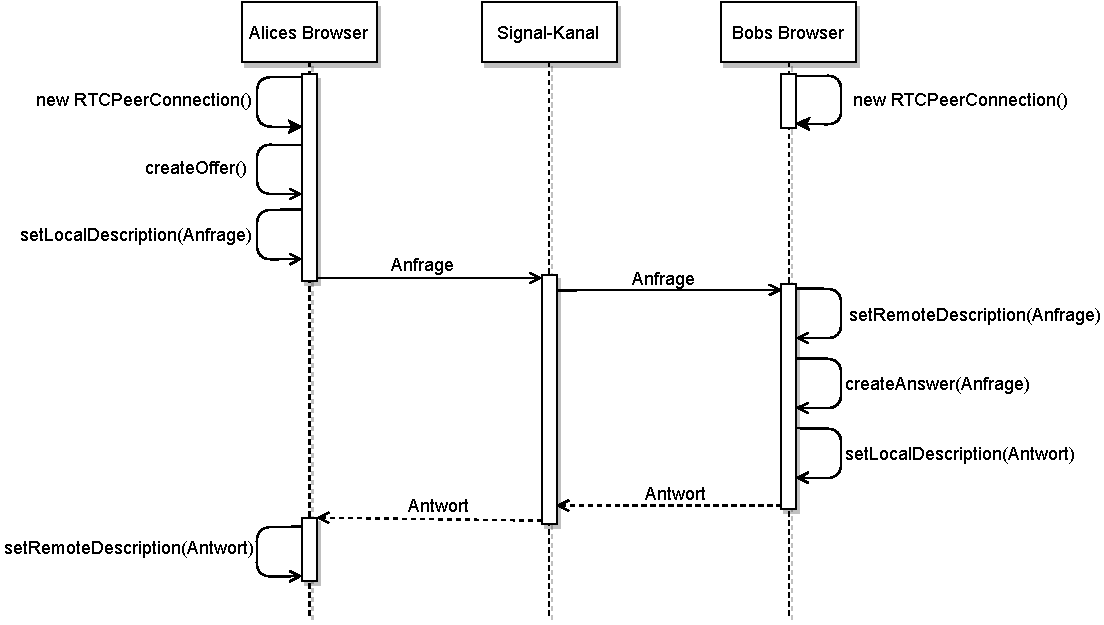
\includegraphics[width=0.89\textwidth]{bilder/PDF_SVG/JSEP.pdf}
\caption{\acs{JSEP}-Verbindungsaufbau.}
\label{fig:jsep}
\end{figure}

Um eine Verbindung aufzubauen, ruft Alice erst \textit{createOffer()} auf. Daraufhin wird ein SDP-Packet (\textit{anfrage}) generiert, welches die lokalen Sitzungsparameter enthält. Alice setzt nun ihre lokale Konfiguration via \textit{setLocalDescription()}. Das \acs{SDP}-Packet wird über einen nicht vorgegebenen Signalkanal zu Bob gesendet. Dieser setzt daraufhin die externe Konfiguration seiner Verbindung via \textit{setRemoteDescription()}, und ruft daraufhin die Funktion \textit{createAnswer(anfrage)} auf, welche eine Antwort (\textit{antwort}) generiert. Bob setzt seine lokale Konfiguration, und sendet die Antwort zurück zu Alice. Zuletzt setzt Alice ihre externe Konfiguration. Damit ist der anfängliche Austausch von Sitzungsparametern abgeschlossen \cite{altanai2014}. \acs{JSEP} regelt dabei nur den Austausch von Konfigurationen zwischen zwei Peers, Informationen über die Verbindung werden über das \acs{ICE}-Framework ausgetauscht \cite{loreto2014}. Der vereinfachte Ablauf des Verbindungsaufbaus ist Abbildung ~\ref{fig:jsep} zu entnehmen.

\subsubsection{STUN: Session Traversal Utilities for NAT}
Das \acf{STUN}-Protokoll wird verwendet, um die öffentliche \acs{IP}-Adresse eines Peers zu ermitteln. Auf Anfrage an einen STUN-Server erhält ein Peer seine Server-Reflexive Transportadresse zurück, welche von externen Peers verwendet werden kann, um Daten an den lokalen Peer zu schicken \cite{stunRFC}.\par

\subsubsection{TURN: Traversal Using Relays around NAT}
Im Gegensatz zu Client-Server-Verbindungen, welche nur vom Client eröffnet werden können, kann eine Peer-To-Peer Verbindung sowohl vom lokalen Peer, als auch von einem Peer außerhalb des lokalen Subnetzes eröffnet werden. Hier besteht das Problem, dass nicht jede Art von \acs{NAT} eine solche Interaktion erlaubt \cite{natproblemsRFC}. In solchen Fällen muss ein \acf{TURN}-Server verwendet werden. Ein \acs{TURN}-Server agiert als ein zwischen den Peers liegender Relais-Server, für Fälle, in denen eine direkte Verbindung zwischen Peers aufgrund von \acs{NAT}-Einschränkungen nicht möglich ist.

\subsubsection{ICE: Interactive Connectivity Establishment}
Das \acf{ICE}-Framework erlaubt es Browsern (Peers), Verbindungen untereinander aufzubauen. Es wird benötigt, da dies aufgrund der Tatsache, dass sich Peers in der Regel in einem lokalen Subnetz hinter einem \acs{NAT} (Network Address Translation) befinden, nicht ohne weiteres möglich ist. Das \acs{ICE}-Framework bietet in Kombination mit den Protokollen \acs{STUN} und \acs{TURN} Möglichkeiten, direkte Verbindungen zweier Peers durch \acs{NAT} herzustellen, beziehungsweise Datenverkehr über ein Relais umzuleiten.\par

Eine RTCPeerConnection besitzt immer einen \acs{ICE}-Agenten. Einer der Agenten einer Verbindung agiert als der kontrollierende, der Andere als der kontrollierte Agent. Der kontrollierende Agent hat die Aufgabe, das \acs{ICE}-Kandidatenpaar, welches für die Verbindung genutzt werden soll, auszuwählen. Ein \acs{ICE}-Kandidat beinhaltet Informationen -- im \acs{SDP}-Format -- über Transportadressen, über welche ein Peer erreicht werden kann. Ein \acs{ICE}-Kandidatenpaar ist ein Paar von zwei \acs{ICE}-Kandidaten, welche zum gegenseitigen Verbindungsaufbau zweier Peers verwendet werden können.

\begin{figure}[h]
\centering
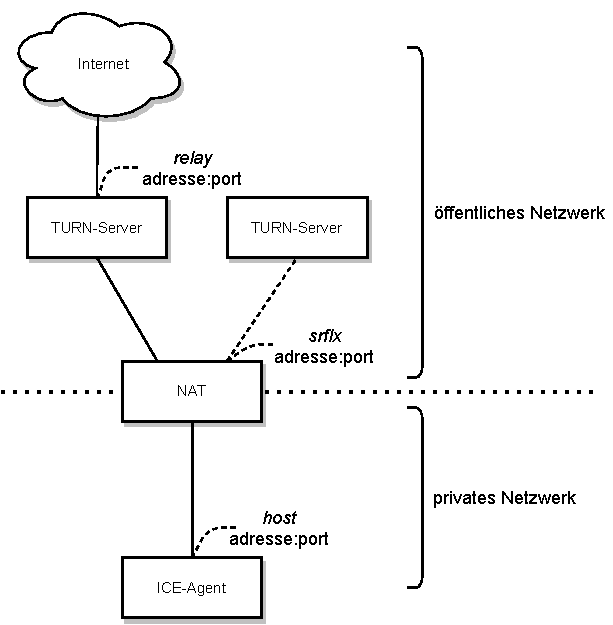
\includegraphics[width=0.80\textwidth]{bilder/PDF_SVG/CANDIDATES_OLD.pdf}
\caption{Diagramm der verschiedenen \acs{ICE}-Kandidaten.}
\source{Nach RFC5245, Abb. 2}
\label{fig:icecandidates}
\end{figure}

Ein Gerät hinter einem \acs{NAT} besitzt keine eigene, öffentliche \acs{IP}-Adresse. Ein Peer muss jedoch seine eigene, öffentliche \acs{IP}-Adresse kennen, um dem Verbindungspartner mitteilen zu können, an welche Adresse dieser die Daten schicken soll. In der Regel handelt es sich bei \acs{ICE}-Kandidaten um \acs{UDP}-Transportadressen. Es existieren zwar auch \acs{TCP}-Kandidaten, diese werden allerdings nicht von allen Browsern unterstützt und in der Regel nicht verwendet. Wie aus Abbildung ~\ref{fig:icecandidates} zu entnehmen, werden primär drei Arten an \acs{UDP}-\acs{ICE}-Kandidaten verwendet:

\begin{itemize}
	\item Ein \textbf{Host}-Kandidat (\textit{typ host}) ist der tatsächliche Adress-Port-Tupel eines Peers. Host-Kandidaten können nur dann verwendet werden, wenn der Peer eine öffentliche \acs{IP}-Adresse besitzt, oder sich sowohl der lokale, als auch externe Peer im gleichen Subnetz, oder auf dem gleichen Gerät befinden.
	\item Ein \textbf{Server-Reflexiver}-Kandidat (\textit{typ srflx}) repräsentiert die öffentliche \acs{IP}-Adresse eines Peers, also die öffentliche \acs{IP}-Adresse des \acs{NAT}s, hinter welchem sich der Peer befindet.
	\item Ein \textbf{Relais}-Kandidat (\textit{typ relay}) ist ein Adress-Port-Tupel, welcher dem Peer von einem \acs{TURN}-Server zugeordnet wurde. Diese Adresse ist dabei die Adresse, welche der \acs{TURN}-Server nutzt, um eingehende Daten an den Peer, und ausgehende Daten von dem Peer weiterzuleiten.
\end{itemize}

Die \acs{STUN} und \acs{TURN} Server lassen sich beim Erstellen der RTCPeerConnection konfigurieren. \acs{WebRTC} prüft die Verbindung zu allen möglichen \acs{ICE}-Kandidaten eines Peers asynchron und parallel, sobald die lokale Beschreibung einer Verbindung gesetzt ist. Dieser Prozess -- der sogenannte \glqq{}\acs{ICE}-Sammelprozess\grqq{} -- setzt eine Kommunikation mit \acs{STUN}- und \acs{TURN}-Servern vorraus und kann daher, je nach Latenz und Antwortzeit der Server, einige Zeit beanspruchen.\par

Aus diesem Grund ermöglicht es \acs{WebRTC}, \acs{ICE}-Kandidaten zu \glqq{}tricklen\grqq{}, also jeweils einzelne Kandidaten bei Erhalt einer Serverantwort an den externen Peer zu schicken. Dies optimiert den Vorgang des Austauschs von \acs{ICE}-Kandidaten, da der \acs{JSEP}-Anfrage-Antwort-Prozess parallel zum \acs{ICE}-Sammelprozess stattfinden kann.\par

\vspace{1pc}
\lstset{style=STYLE_ICE_CANDIDATE_0}
\begin{lstlisting}[caption={SDP-Datenstring eines Relais-ICE-Kandidaten},captionpos=b,label={lst:candidate}]
candidate:1411127089 1 udp 33562367 <@\textcolor{blue}{20.56.95.156}@> <@\textcolor{blue}{12926}@> <@\textcolor{red}{typ}@> <@\textcolor{red}{relay}@> raddr 0.0.0.0 rport 0 generation 0 ufrag uVtu network-cost 999
\end{lstlisting}

Jede RTCPeerConnection besitzt daher die Rückruffunktion \glqq{}$onicecandidate$\grqq{}, welche bei Erhalt eines neuen \acs{ICE}-Kandidaten aufgerufen wird. Die Parameter dieser Rückruffunktion enthalten die \acs{SDP}-Daten des Kandidaten. Die Struktur dieser Daten ist Beispielhaft Abbildung~\ref{lst:candidate} zu entnehmen. Dabei handelt es sich um einen \acs{UDP}-Relais-Kandidaten, zu erkennen am \glqq{}typ relay\grqq{}, hervorgehoben in Rot. Die Adresse und der Port sind in Blau hervorgehoben. Nachdem diese Daten an den externen Peer gesendet wurden, muss der Kandidat auf der Empfängerseite über die $addIceCandidate$-Funktion der RTCPeerConnection hinzugefügt werden.

\subsubsection{SCTP: Stream Control Transmission Protocol}
Zur Übertragung von Daten via RTCDataChannels nutzt \acs{WebRTC} das \acf{SCTP}. Der \acs{SCTP} Standard wurde erstmals im Jahre 2000 von der \acs{IETF} veröffentlicht, und seitdem weiterentwickelt und erweitert. \acs{SCTP} ist ein nachrichtenorientiertes Transportprotokoll, welches im \acf{OSI}-Referenzmodell, ähnlich dem \acf{UDP} und dem \acf{TCP}, auf der Transportschicht liegt. Das Protokoll arbeitet dabei basierend auf verbindungslosen Netzwerkprotokollen, wie dem \acf{IP} \cite{sctpRFC}.\par

Im Gegensatz zu \acs{TCP} und \acs{UDP} lassen sich bei \acs{SCTP}, je nach gewünschter Verbindungsart, die folgenden Aspekte konfigurieren:
\begin{itemize}
	\item\textbf{Reihenfolge}: \acs{SCTP} ermöglicht es, sowohl geordnete, als auch ungeordnete Datenströme aufzubauen \cite{sctpRFC}.
	\item\textbf{Zuverlässigkeit}: Die Zuverlässigkeit der Paketlieferungen ist auf zwei Arten konfigurierbar. Es ist möglich, eine maximale Anzahl an Versuchen festzulegen, mit welcher versucht wird, ein Datenpaket zu versenden. Zudem kann eine maximale Lebenszeit für Pakete angegeben werden. Ist diese Lebenszeit, das sogenannte 'Retransmission Timeout' für eine Paketsendung abgelaufen, so wird kein weiterer Versuch unternommen, das Paket abzuschicken \cite{sctpRFC}.
\end{itemize}

\vspace{11pt}

Im Gegensatz zu \acs{TCP} und \acs{UDP} ermöglicht \acs{SCTP} Multiplexing auf Basis von mehreren, separaten sowie parrallelen Datenströmen innerhalb einer Verbindung. Dazu ist der Datenteil eines \acs{SCTP}-Packets in sognenannte \glqq{}Chunks\grqq{}  aufgeteilt, wobei Daten-Chunks jeweils einem Datenstrom zugeordnet werden können \cite{sctpRFC}.\par

\begin{table}[ht]
\centering
\begin{tabular}[t]{lccc}
\toprule
&TCP&UDP&SCTP\\
\midrule
Nachrichtenordnung&Geordnet&Ungeordnet&Konfigurierbar\\
Zuverlässigkeit&Zuverlässig&Unzuverlässig&Konfigurierbar\\
Flusskontrolle&Ja&Nein&Ja\\
Überlastkontrolle &Ja&Nein&Ja\\
Mehrere Datenströme&Nein&Nein&Ja\\
\bottomrule
\end{tabular}
\caption{Vergleich von \acs{TCP} und \acs{UDP} mit \acs{SCTP}.}
\label{table:vergleichNetzwerkProtokolle}
\end{table}

Ein direkter Vergleich der drei Protokolle lässt sich aus Tabelle~\ref{table:vergleichNetzwerkProtokolle} entnehmen. Im Gegensatz zu \acs{UDP} bietet \acs{SCTP} außerdem Fluss- und Überlastkontrolle. Damit gestaltet sich \acs{SCTP} weitaus flexibler als die beiden gängigsten Transportprotokolle.\par

%\begin{figure}[h]
%\centering
%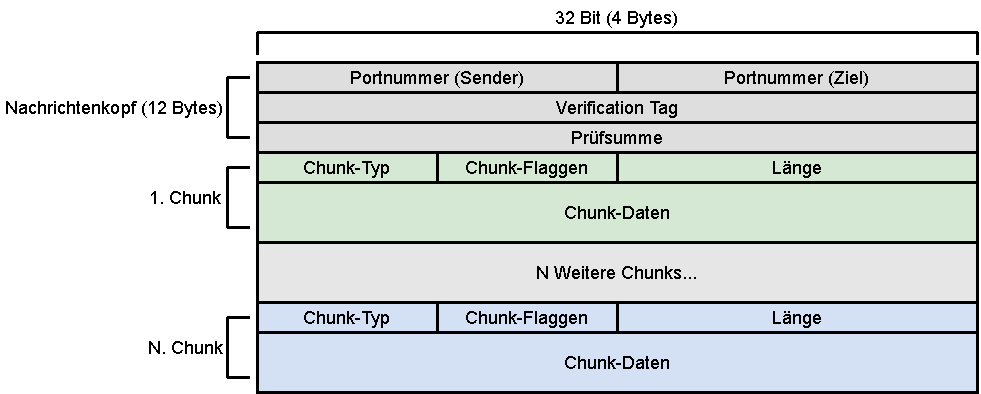
\includegraphics[width=0.95\textwidth]{bilder/PDF_SVG/SCTP_PACKET.pdf}
%\caption{Aufbau eines \acs{SCTP}-Packets.}
%\label{fig:sctpPacket}
%\end{figure}

%Ein \acs{SCTP}-Packet besteht aus einem Kopf- und einem Datenteil. Der Kopfteil beinhaltet neben dem Quell- und Zielport, sowie einer Prüfsumme noch ein \glqq{}Verification Tag\grqq{}, welches verwendet wird, um auf der Empfängerseite den Absender des Packets zu verifizieren, und eingehende Packete von denen früherer Verbindungen zu unterscheiden \cite{sctpRFC}.

%Der Datenteil des Packets ist in sogenannte \glqq{}Chunks\grqq{}  aufgeteilt. Jedes \glqq{}Chunk\grqq{} besitzt dabei Informationen wie den Chunk-Typ, die Länge in Bytes, oder die Zugehörigkeit zu Datenströmen. Insgesamt existieren über 14 Chunk-Typen, von einfachen Daten-Chunks zu Chunks, welche Daten zur Kontrolle der Verbindung beinhalten \cite{sctpRFC}. Je nach verwendeten Erweiterungen des \acs{SCTP}-Protokolls kann die Anzahl der Chunk-Typen variieren. Alle Arten dieser \glqq Chunks\grqq{} zu beschreiben würde den Rahmen dieser Arbeit überschreiten. Die generelle Struktur eines Datenpackets ist Abbildung ~\ref{fig:sctpPacket} zu entnehmen. Die maximale größe eines \glqq{}Chunks\grqq{} ist dabei, aufgrund des zwei-Byte langen Längenfelds auf 65,535 Kilobyte limitiert.

\subsubsection{DTLS: Datagram Transport Layer Security}
Das \acf{DTLS}-Protokoll ist ein auf \acf{TLS} aufbauendes Protokoll zur Verschlüsselung von Daten in auf Datengramm-basierenden Verbindungen. Im Gegensatz zu \acs{TLS}, welches für die Nutzung mit \acs{TCP} konzipiert wurde, kann \acs{DTLS} also über \acs{UDP} übertragen werden.\par

Die \acs{SCTP}-Verbindung eines Datenkanals läuft nicht direkt auf dem \acf{IP}. Da das von Datenkanälen genutzte \acs{SCTP}-Protokoll über keine eigene Verschlüsselung verfügt, und Verschlüsselung aller Daten eine zentrale Anforderung von \acs{WebRTC} darstellt, werden Daten über einen \acs{DTLS}-Tunnel -- welcher wiederrum über \acs{UDP} liegt -- zwischen den Verbindungspartnern ausgetauscht \cite{rtcsecurity}. Im Gegensatz zu \acs{SCTP} bietet \acs{SRTP} eigene Verschlüsselung, und kann auch ohne \acs{DTLS}-Tunnel verwendet werden. Wann welche Konfiguration verwendet wird ist dabei je Implementation in Browser oder Anwendung unterschiedlich (vgl. Abbildung~\ref{fig:protocols}).

\section{Node.js}
Node.js ist eine kostenlose, plattformunabhängige JavaScript Laufzeitumgebung.
Diese ermöglicht das Ausführen von JavaScript Programmen außerhalb eines Browsers, zum Beispiel auf einem Server. Node.js ist Open-Source und kann kostenlos verwendet werden. Programme setzen sich aus sogenannten \textit{modules}, zu Deutsch Modulen, zusammen. Ein Modul kann dabei jegliche Funktionalität, wie zum Beispiel Klassen, Funktionen und Konstanten exportieren, welche dann wiederrum von weiteren Modulen oder Programmen verwendet werden können. Module können über das \textit{require}-Stichwort geladen werden. Node.js bietet integrierte Webserver-Funktionalität via dem \acf{HTTP}-Modul, welches das Erstellen eines Webservers ermöglicht \cite{nodejs}. Weiterhin bietet Node.js mit dem \glqq{}crypto\grqq{}-Modul kryptografische Funktionen, welche auf OpenSSL (Open Secure Socket Layer) basieren.\par 

Node.js ist in den Repositories aller aktuellen Linux-Distributionen enthalten\footnote{Weitere Informationen: \url{https://nodejs.org/en/download/package-manager/}}, und kann mit den entsprechenden Packetmanagern, beziehungsweise über die Website\footnote{Node.js Downloads: \url{https://nodejs.org/en/download/}} heruntergeladen und installiert werden.\par

\subsection{NPM: Node Package Manager}
Zur Verwaltung und zum Teilen von Packeten nutzt Node.js den \ac{NPM}. Ein Packet sind in diesem Kontext ein oder mehrere Module, gekoppelt mit allen Dateien, welche diese benötigen. Packete werden auf \textit{npmjs.com} gehostet. Die Liste der von einem Projekt verwendeten Module wird in der Datei \textit{package.json} gespeichert.

\subsection{Verwendete Node-Packete}
Neben den standartmäßig in Node.js enthaltenen \glqq{}http\grqq{}- und \glqq{}crypto\grqq{}-Modulen werden zwei weitere Packete genutzt: die \glqq{}socket.io\grqq{} Bibliothek und das \glqq{}express\grqq{}-Framework.

\subsubsection{socket.io}
\glqq{}socket.io\grqq{} ist eine Bibliothek, welche bidirektionale Echtzeitkommunikation zwischen einem Client und einem Server ermöglicht. Dazu nutzt Socket.io intern WebSockets\cite{socketio}. Ein WebSocket ermöglicht Kommunikation zwischen einem Client und einem Server. Der Datenaustausch findet dabei über das \ac{TCP} statt \cite{websocketRFC}. Das WebSocket \ac{API} wird von allen aktuellen Browsern unterstützt\footnote{vgl. \url{https://caniuse.com/mdn-api_websocket}, Stand: 08.04.2021}. Socket.io läuft auf einem Node.js Server \cite{socketio}.\par

Die Kommunikation zwischen Client und Server wird bei Socket.io über Events geregelt. Client und Server können Events -- definiert durch einen String -- mit angehängten Daten emittieren. Basierend auf dem Event-String wird dann auf der Empfängerseite eine Rückruffunktion aufgerufen, vorrausgesetzt diese ist definiert. Die Daten werden der Rückruffunktion als Parameter übergeben. Socket.io ermöglicht auf der Serverseite sowohl das Broadcasting an alle, beziehungsweise an ein Subset an Clients, als auch Unicasting an einen spezifischen Client \cite{socketio}.\par

Die Socket.io Bibliothek ist in eine Client-, und eine Serverseitige Bibliothek aufgeteilt. Die Clientseitige Bibliothek ermöglicht das Verbinden mit einem Node.js Server. Ein Client kann sowohl Events mit Daten emittieren, als auch Rückruffunktionen registrieren, mit welchen der Client Daten vom Server empfangen kann. Auf der Serverseite ist es möglich, bei Verbindungsaufbau Rückruffunktionen für einen neu verbundenen Client zu registrieren, welche bei dem Eingang von Daten je nach Event-Typ aufgerufen werden. Der Server kann ebenfalls Events an Clients emittieren.

\subsubsection{express}
\glqq{}express\grqq{} ist ein Node-Web-Framework, welches bei der Erstellung von Webanwendungen zum Einsatz kommt. Express agiert als Middleware zwischen einem \acs{HTTP}-Server und einer Webanwendung und ermöglicht es, basierend auf \acs{HTTP}-Methoden und \acf{URL}s -- den sogenannten \glqq{}Pfaden\grqq{} -- verschiedene Aktionen auszuführen \cite{express}. Zudem bietet express weitere Funktionalitäten, wie das Bereitstellen von statischen Website-Daten, oder die Integration von \glqq{}Rendering-Engines\grqq{}, welche die Daten einer Website je nach Pfad dynamisch anpassen \cite{express}.